\documentclass[fleqn,10pt]{wlscirep}
\usepackage[utf8]{inputenc}
\usepackage[T1]{fontenc}
\usepackage{array}
\usepackage{tabularray}
\usepackage{stringstrings}
%%comandos nuevos
\newcommand{\firmante}{1}
\newcommand{\thedate}{ 22 de mayo de 2025}
\newcommand{\memorando}{EPN-DOCDCTA-2025-0055-M}
\newcommand{\docente}{PhD. Roque Antonio Santos Torres}
\newcommand{\masculino}{1}
\newcommand{\departamento}{Departamento de Ciencias Nucleares}
\newcommand{\cargo}{Profesor Agregado a Tiempo Completo }
\newcommand{\onlyScopus}{0} % 1 Only Scopus, 0 All
\newcommand{\onlyEpnScopusAffil}{0} % 1 Only EPN
\newcommand{\onlyEpnRegionalAffil}{1} % 1 Only EPN
\newcommand{\onlyEpnMemoriasAffil}{1} % 1 Only EPN
\newcommand{\onlyEpnCapsAffil}{1} % 1 Only EPN
\newcommand{\doi}[3][gray]{\href{#2}{\color{#1}{#3}}}

%%SCOPUS
\newcommand{\numpublicacionesscopus}{10 }
%% 6 Artículos, 4 Artículos de Conferencia, 2 Capitulos de Libros y 1 Review
\newcommand{\distribucionArticulosScopus}{9 Artículos y 1 Articulo de Conferencia}
\newcommand{\areasTematicasITEM}
{
\item Physics and Astronomy
\item Engineering
\item Chemistry
\item Environmental Science
\item Earth and Planetary Sciences
\item Energy
\item Materials Science
\item Mathematics
\item Multidisciplinary








}
\newcommand{\numAreasTematicas}{9 }

\newcommand{\detalleScopus}
{
 
\item (2023) "e-RPT: Ecuadorian radioactive particle tracking. Proposal and evaluation of a low-budget RPT system with GEANT4". Applied Radiation and Isotopes. \textbf{Indexada en SCOPUS - Radiation (Q3)}.\doi{https://doi.org/10.1016/j.apradiso.2023.110754}{ DOI: 10.1016/j.apradiso.2023.110754}
\item (2023) "SAS GEANT4 application and machine learning algorithms for radioactive particle tracking". Radiation Physics and Chemistry. \textbf{Indexada en SCOPUS - Radiation (Q2)}.\doi{https://doi.org/10.1016/j.radphyschem.2023.111056}{ DOI: 10.1016/j.radphyschem.2023.111056}
\item (2022) "Simulation of a HPGe Detector with GEANT4". Revista Politecnica. \textbf{Indexada en SCOPUS - Applied Mathematics (Q4); Chemistry (miscellaneous) (Q4); Engineering (miscellaneous) (Q4); Environmental Engineering (Q4); Geochemistry and Petrology (Q4); Geotechnical Engineering and Engineering Geology (Q4); Physics and Astronomy (miscellaneous) (Q4)}.\doi{https://doi.org/10.33333/rp.vol50n2.01}{ DOI: 10.33333/rp.vol50n2.01}
\item (2021) "Ionizing radiation as adjuvant for the abiotic degradation of plastic bags containing pro-oxidant additives". Journal of Applied Polymer Science. \textbf{Indexada en SCOPUS - Chemistry (miscellaneous) (Q2); Materials Chemistry (Q2); Polymers and Plastics (Q2); Surfaces, Coatings and Films (Q2)}.\doi{https://doi.org/10.1002/app.49664}{ DOI: 10.1002/app.49664}
\item (2020) "Viscosity Study in a Crude Oil Additive with Dispersants and Asphaltene Solvent". Revista Politecnica. \textbf{Indexada en SCOPUS - Applied Mathematics; Chemistry (miscellaneous); Engineering (miscellaneous); Environmental Engineering; Geochemistry and Petrology; Geotechnical Engineering and Engineering Geology; Physics and Astronomy (miscellaneous)}.\doi{https://doi.org/10.33333/rp.vol46n2.01}{ DOI: 10.33333/rp.vol46n2.01}
\item \textbf{(2018) "Simulated time-dependent data to estimate uncertainty in fluid flow measurements". Nuclear Engineering and Design. Indexada en SCOPUS - Materials Science (miscellaneous) (Q1); Mechanical Engineering (Q1); Nuclear and High Energy Physics (Q1); Nuclear Energy and Engineering (Q1); Safety, Risk, Reliability and Quality (Q1); Waste Management and Disposal (Q1)}.\doi{https://doi.org/10.1016/j.nucengdes.2018.07.005}{ DOI: 10.1016/j.nucengdes.2018.07.005}
\item \textbf{(2017) "A feature point identification method for positron emission particle tracking with multiple tracers". Nuclear Instruments and Methods in Physics Research Section A Accelerators Spectrometers Detectors and Associated Equipment. Indexada en SCOPUS - Instrumentation (Q1); Nuclear and High Energy Physics (Q2)}.\doi{https://doi.org/10.1016/j.nima.2016.10.057}{ DOI: 10.1016/j.nima.2016.10.057}
\item \textbf{(2017) "Three-dimensional spatiotemporal tracking of fluorine-18 radiolabeled yeast cells via positron emission particle tracking". Plos One. Indexada en SCOPUS - Agricultural and Biological Sciences (miscellaneous) (Q1); Biochemistry, Genetics and Molecular Biology (miscellaneous) (Q1); Medicine (miscellaneous) (Q1)}.\doi{https://doi.org/10.1371/journal.pone.0180503}{ DOI: 10.1371/journal.pone.0180503}
\item (2016) "Tracking synthetic particle paths generated in GATE with multi-positron emission particle tracking (MPEPT)". Transactions of the American Nuclear Society. \textbf{Conferencia Indexada en SCOPUS}. \underline{(Sin Filiación)}
\item \textbf{(2016) "A novel clustering approach to positron emission particle tracking". Nuclear Instruments and Methods in Physics Research Section A Accelerators Spectrometers Detectors and Associated Equipment. Indexada en SCOPUS - Instrumentation (Q1); Nuclear and High Energy Physics (Q2)}.\doi{https://doi.org/10.1016/j.nima.2015.11.136}{ DOI: 10.1016/j.nima.2015.11.136} \underline{(Sin Filiación)}









}


%%WEB OF SCIENCE
\newcommand{\numpublicacionesWos}{0 }
%% 6 Artículos, 1 Review, Artículos de Conferencia y 3 Capítulos de Libros
\newcommand{\distribucionArticulosWos}{1 Artículo y 5 Artículos de Conferencias }

\newcommand{\detalleWos}{
\item (2017) "THE LEARNING STYLE IN LOCAL HIGHER EDUCATION: EXPERIENTIAL MODEL AND CO-CREATION". INTED2017 Proceedings. \textbf{Conferencia Indexada en Conference Proceedings Citation Index (CPCI)}.
\item (2017) "APPROACHING OF ICT IN CO-CREATION OF DIGITAL EDUCATIONAL MATERIALS WITH SUPPORT OF AUTHOR'S TOOLS". EDULEARN17 Proceedings. \textbf{Conferencia Indexada en Conference Proceedings Citation Index (CPCI)}.
\item (2016) "DIGITAL DIVIDE ASSOCIATED WITH ADOPTION OF INFORMATION AND COMMUNICATION TECHNOLOGIES (ICTS) IN SMALL AND MEDIUM BUSINESSES (SMBS)". ICERI2016 Proceedings. \textbf{Conferencia Indexada en Conference Proceedings Citation Index (CPCI)}.
\item (2016) "INTERESTS AND NEEDS IN THE MONITORING FOR GRADUATES. A CASE STUDY". EDULEARN16 Proceedings. \textbf{Conferencia Indexada en Conference Proceedings Citation Index (CPCI)}.
\item (2016) "THE UNIVERSITY AND THE SOCIAL ENTREPRENEURSHIP". INTED2016 Proceedings. \textbf{Conferencia Indexada en Conference Proceedings Citation Index (CPCI)}.
}


%%REGIONALES
\newcommand{\numpublicacionesregionales}{0 }
\newcommand{\detalleRegionales}{
  \item (2024) "LIMITACIONES PARA LA APLICACIÓN DE TECNOLOGÍA SOCIAL EN LA PROTECCIÓN DEL PÁRAMO". Revista Estudios de la Gestión. \textbf{ Indexada en Scielo}. 
  
}

\newcommand{\aniosRegionales}{0 }


%%MEMORIAS
\newcommand{\numMemorias}{0 }
\newcommand{\aniosMemorias}{ }
\newcommand{\detalleMemorias}{
\item (2013) "Inclusive and beneficial? Governance in global food value chains in Costa Rica". 138th EAAE Seminar on Pro-poor Innovations in Food Supply Chains, Ghent Belgium. \textbf{ No se puede verificar la indexación}.
}


%%LIBROS Y CAP. LIBROS
\newcommand{\numLibros}{0 }
\newcommand{\detalleLibros}{
  \item (2017) "Ecuador". Challenges and Opportunities for Food and Nutrition Security for the Americas: The vision of the Academies of Sciences. \textbf{ Cap. Libro}.
}


%%Publicaciones 5 años de todo 2015-2019
\newcommand{\numpublicacionescincoaios}{555555555 }


\newcommand{\numTotalPubRegyScopus}{10 }

\renewcommand{\figurename}{Figura}
\addto\captionsenglish{\renewcommand{\figurename}{Figura}}
%\DeclareUnicodeCharacter{202F}{$\mu$}
\renewcommand{\tablename}{Tabla}
\addto\captionsenglish{\renewcommand{\tablename}{Tabla}}

\title{Certificación de Publicaciones\small\hfill\thedate}
\author[]{\docente}
\affil[]{\departamento}
\affil[]{Escuela Politécnica Nacional}

%\affil[*]{corresponding.author@email.example}

%\affil[+]{these authors contributed equally to this work}

%\keywords{Keyword1, Keyword2, Keyword3}

\begin{abstract}
\stringlength[q]{\memorando}
\ifnum\theresult>0 {El presente informe se realiza en base a la solicitud del memorando \memorando, con la finalidad de certificar \ifnum\numTotalPubRegyScopus>1{las publicaciones }\else{la publicación }\fi \ifnum\masculino=1{del profesor }\else{de la profesora }\fi \docente. } \else {El presente informe se realiza con la finalidad de certificar \ifnum\numTotalPubRegyScopus>1{las publicaciones }\else{la publicación}\fi \ifnum\masculino=1{del profesor }\else{de la profesora }\fi \docente.} \fi
\end{abstract}
\begin{document}

\flushbottom
\maketitle
\noindent{\parbox{\dimexpr\linewidth-2\fboxsep\relax}{\color{color1}\large\sffamily\textbf{INFORME TÉCNICO\\}}}
% * <john.hammersley@gmail.com> 2015-02-09T12:07:31.197Z:
%
%  Click the title above to edit the author information and abstract
%
\thispagestyle{empty}

\noindent El presente informe se realiza en base a la información recopilada por la Dirección de Investigación, de \ifnum\numpublicacionesscopus>0{la base de datos científicos Scopus\ifnum\numpublicacionesregionales>0{ y }\fi}\fi \ifnum\numpublicacionesregionales>0{bases de datos indexadas}\fi.


\ifnum\numpublicacionesscopus>0{
\section*{Publicaciones Scopus}
\subsection*{Tipo y Número de publicaciones Scopus \ifnum\masculino=1{del }\else{de la }\fi \docente}
\vspace{1mm}
\ifnum\masculino=1{El }\else{La }\fi \docente, es \cargo  de la Escuela Politécnica Nacional y miembro del \departamento. \\\\Ha  participado  en  un  total  de \numpublicacionesscopus \ifnum\numpublicacionesscopus>1{publicaciones Scopus como \ifnum\masculino=1{autor/co-autor }\else{autora/co-autora }\fi de las mismas, distribuidas en \distribucionArticulosScopus}\else{publicación Scopus como \ifnum\masculino=1{autor/co-autor }\else{autora/co-autora }\fi de la misma, siendo \distribucionArticulosScopus }\fi. Tal como se detalla a continuación:
\begin{enumerate}
\detalleScopus
\end{enumerate}
\ifnum\onlyEpnScopusAffil=0{Sin Filiación: Publicación sin filiación de la Escuela Politécnica Nacional. }\fi

\vspace{5mm}

\ifnum\numpublicacionesscopus>1{ \noindent Adicionalmente, en la Figura \ref{fig:gr1} se muestra la tendencia por año de las publicaciones en Scopus \ifnum\masculino=1{del }\else{de la }\fi \docente :

\begin{figure}[ht]
\centering
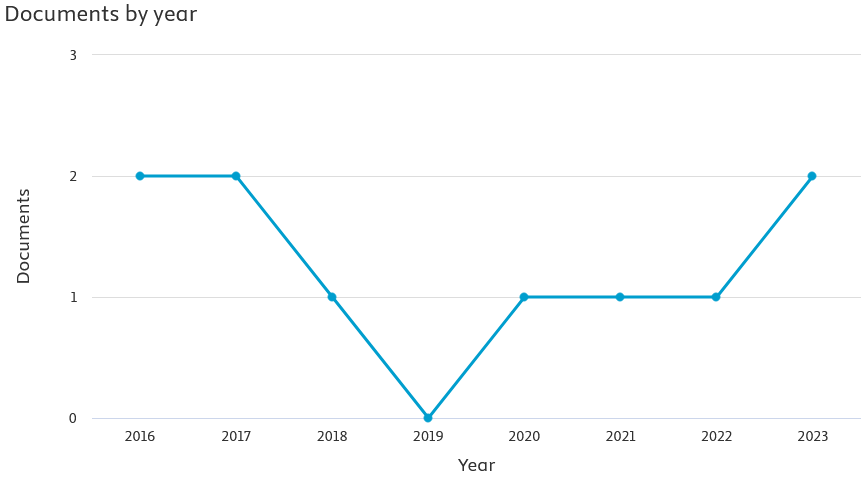
\includegraphics[width=.95 \linewidth]{gr1}%.8
\caption{\small Publicaciones Scopus por Año - Fuente web de Scopus.}
\label{fig:gr1}
\end{figure}
}\fi
\vspace{1mm}
%\newpage %usar si areas se anteponen al grafico
\subsection*{Áreas Temáticas de publicaciones Scopus \ifnum\masculino=1{del }\else{de la }\fi \docente}
\vspace{1mm}
\ifnum\masculino=1{El }\else{La }\fi \docente, ha publicado en \numAreasTematicas \ifnum\numAreasTematicas>1{áreas temáticas, las cuales se detallan }\else{área temática, la cual se detalla }\fi a continuación:
\begin{enumerate}
\areasTematicasITEM
\end{enumerate}
}\fi


\ifnum\numpublicacionesWos>0{
\vspace{3mm}
\section*{Publicaciones Web of Science}
\subsection*{Tipo y Número de publicaciones Web of Science \ifnum\masculino=1{del }\else{de la }\fi \docente}
\vspace{1mm}
Ha  participado  en  un  total  de \numpublicacionesWos \ifnum\numpublicacionesWos>1{publicaciones indexadas en la Web of Science Core Collection como \ifnum\masculino=1{autor/co-autor }\else{autora/co-autora }\fi de las mismas, distribuidas en \distribucionArticulosWos}\else{publicación indexada en la Web of Science Core Colection como \ifnum\masculino=1{autor/co-autor }\else{autora/co-autora }\fi de la misma, siendo \distribucionArticulosScopus }\fi. Tal como se detalla a continuación:
\begin{enumerate}
\detalleWos
\end{enumerate}
\vspace{2mm}
\ifnum\onlyEpnScopusAffil=0{Sin Filiación: Publicación sin filiación de la Escuela Politécnica Nacional.}\fi
}\fi


\ifnum\numpublicacionesregionales>0{
\section*{Otras Indexaciones}
\ifnum\numpublicacionesscopus<1{\ifnum\masculino=1{El }\else{La }\fi \docente, es \cargo  de la Escuela Politécnica Nacional y miembro del \departamento. \\\\}\fi
\ifnum\masculino=1{El }\else{La }\fi \docente, cuenta con \numpublicacionesregionales \ifnum\numpublicacionesregionales>1{indexaciones, como se detallan a continuación}\else{artículo indexado, como se detalla a continuación}\fi:
\begin{enumerate}
\detalleRegionales
\end{enumerate}
\vspace{0mm}
}\fi
\ifnum\onlyEpnRegionalAffil=0{Sin Filiación: Publicación sin filiación de la Escuela Politécnica Nacional. }\fi

\ifnum\numMemorias>0{
\section*{Memorias de Eventos Científicos}
\ifnum\masculino=1{El }\else{La }\fi \docente, cuenta con \numMemorias \ifnum\numMemorias>1{publicaciones en memorias de eventos científicos, como se detallan a continuación}\else{publicación en memorias de eventos científicos, como se detalla a continuación }\fi:
\begin{enumerate}
\detalleMemorias
\end{enumerate}
\vspace{1mm}
\ifnum\onlyEpnMemoriasAffil=0{Sin Filiación: Publicación sin filiación de la Escuela Politécnica Nacional. }\fi
}\fi

\ifnum\numLibros>0{
\section*{Libros y Capítulos de Libros}
\ifnum\masculino=1{El }\else{La }\fi \docente , cuenta con \numLibros \ifnum\numLibros>1{publicaciones en Libros y Capítulos de Libros, como se detallan a continuación}\else{publicación en Libros y Capítulos de Libros, como se detalla a continuación}\fi:
\begin{enumerate}
\detalleLibros
\end{enumerate}
\vspace{1mm}
\ifnum\onlyEpnCapsAffil=0{Sin Filiación: Publicación sin filiación de la Escuela Politécnica Nacional. }\fi
}\fi

%\newpage
\section*{Conclusión}

Por los antecedentes expuestos, \ifnum\firmante=1{la Dirección de Investigación }\else{el Vicerrectorado de Investigación, Innovación y Vinculación }\fi de la Institución, certifica que \ifnum\masculino=1{el }\else{la }\fi \docente, cuenta con un total de \numTotalPubRegyScopus \ifnum\numTotalPubRegyScopus>1{publicaciones Scopus.}\fi \\
% y \numpublicacionesregionales artículos indexados.}\else{\ifnum\numpublicacionesscopus=1{publicación Scopus.}\fi \ifnum\numpublicacionesregionales=1{artículo regional.}\fi \ifnum\numMemorias=1{ memoria de eventos científicos.}\fi \ifnum\numLibros=1{ Libro, Captítulo de Libro.}\fi }\fi \\

%Por los antecedentes expuestos, \ifnum\firmante=1{la Dirección de Investigación }\else{el Vicerrectorado de Investigación, Innovación y Vinculación }\fi de la Institución, certifica que \ifnum\masculino=1{el }\else{la }\fi \docente, cuenta con un total de \numTotalPubRegyScopus \ifnum\numTotalPubRegyScopus>1{publicaciones, de las cuales \numpublicacionesscopus son Scopus y \numMemorias memoria de eventos científicos.}\else{\ifnum\numpublicacionesscopus=1{publicación Scopus.}\fi \ifnum\numpublicacionesregionales=1{artículo regional.}\fi \ifnum\numMemorias=1{ memoria de eventos científicos.}\fi \ifnum\numLibros=1{ Libro, Captítulo de Libro.}\fi }\fi \\

%Por los antecedentes expuestos, el Vicerrectorado de Investigación, Innovación y Vinculación de la Institución, certifica que \ifnum\masculino=1{el }\else{la }\fi \docente, cuenta con un total de \numTotalPubRegyScopus \ifnum\numTotalPubRegyScopus>1{publicaciones, de las cuales \numpublicacionesscopus son Scopus, \numpublicacionesregionales son artículos regionales, \numMemorias son memorias de eventos científicos, 1 Capítulo de Libro y 1 Libro.}\else{\ifnum\numpublicacionesscopus=1{publicación Scopus.}\fi \ifnum\numpublicacionesregionales=1{artículo regional.}\fi \ifnum\numMemorias=1{ memoria de eventos científicos.}\fi \ifnum\numLibros=1{ Libro, Captítulo de Libro.}\fi }\fi \\

\noindent \ifnum\masculino=1{El }\else{La }\fi \docente\hspace{0.3em}puede hacer uso del presente certificado para lo que considere necesario.
 \\
\vfill
\ifnum\firmante>1{
\noindent \textbf{Dr. Marco Oswaldo Santórum Gaibor} \\
\textbf{VICERRECTOR DE INVESTIGACIÓN, INNOVACIÓN Y VINCULACIÓN DE LA ESCUELA POLITÉCNICA NACIONAL}
}\else{
\noindent \textbf{Dra. María Monserrate Intriago Pazmiño} \\
\textbf{DIRECTORA DE INVESTIGACIÓN DE LA ESCUELA POLITÉCNICA NACIONAL}
}\fi
\noindent
\begin{table}[ht]
\begin{tabular}{|l|l|}
\hline
\small Elaborado por: & M. Vásquez\\
\hline
\end{tabular}
\end{table}
%\begin{tblr} {
%  colspec = {|Q[c,c]|Q[c,m]|Q[r,10em]|},
%  stretch = 6pt,
%  rowsep = 0pt,
%  hlines = {black, 0.5pt},
%  vlines = {black, 0.5pt},
%}
%Elaborado por: &  R. Villarroel &  \\
%\end{tblr}
\end{document}